\documentclass{article}
\usepackage[margin = 0.15in,landscape]{geometry}
%\usepackage{wasysym}
\usepackage{multicol}
\usepackage{array}
\usepackage{amsmath}
\usepackage{amssymb}
\usepackage{lmodern}
\usepackage{graphicx}
\usepackage{enumitem}
\usepackage{mathrsfs}
\setlength\parindent{0pt}
\renewcommand{\baselinestretch}{0.75}




\begin{document}
\begin{multicols*}{3}
    Marissa Palamara\par 
    ASEN 3128\par 
    Spring 2021
    \vspace{-0.5cm}
    \setlist{nolistsep}

% ---------- Concepts ---------- %
\section*{Nomenclature}
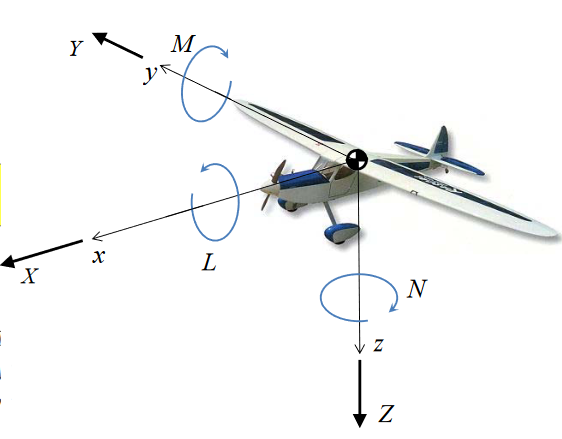
\includegraphics[width=0.75\linewidth]{Images/Body_Frame.png}\par
$\mathbf{V}_B^E = $ velocity in intertial frame written in body coordinate system\par 
$\mathbf{F}_B^{aero}= X\mathbf{e}_x+Y\mathbf{e}_y+Z\mathbf{e}_z=[X;Y;Z]$\par 
$\mathbf{M}_B^{aero}=\mathbf{G}_B^{aero}=L\mathbf{e}_x+M\mathbf{e}_y+N\mathbf{e}_z=[L;M;N]$\par 
$\mathbf{V}_B^E=u^E\mathbf{e}_x+v^E\mathbf{e}_y+w^E\mathbf{e}_z=[u^E;v^E;w^E]$\par 
$V_g=|\mathbf{V}_B^E|=\mathbf{V}_E^E=\sqrt{(u^E)^2+(v^E)^2+(w^E)^2}$\par 
$\mathbf{\omega}_B^E=p^E\mathbf{e}_x+q^E\mathbf{e}_y+r^E\mathbf{e}_z=[p;q;r]$\par 
\subsection*{Four Control Surfaces}
\textbf{Rudder}: $+\delta_r$ = towards -y = negative moment \& positive force\par 
\textbf{Elevator}: $+\delta_e$ = down = negative moment \& negative force\par 
\textbf{Aileron}: $+\delta_a$ = right (+y) down = negative moment\par 
\textbf{Throttle}: $+\delta_t$ = no moment, positive force.\par 
\subsection*{Wind}
\textbf{Background Wind}: $\mathbf{V}^E=\mathbf{V}+\mathbf{W}$
\textbf{Wind Angles}:\par 
$V = |\mathbf{V}_B|$\par
$a=\arctan{\frac{w}{u}}$, $\beta=\arcsin{\frac{v}{V}}$\par 
$u = V\cos{\beta}\cos{\alpha}$, $v=V\sin{\beta}$, $w=V\cos{\beta}\sin{\alpha}$\par 
$\alpha$ = angle of attack, $\beta$ = sideslip angle
% ---------- Euler Angles ---------- %
\section*{Euler Angles}
$R_E^B(\phi,\theta,\psi)=R_{v2}^B(\phi)R_{v1}^{v2}(\theta)R_E^{v1}(\psi)$\par 
Body to Inertial Frame Transformation:\par 
$\mathbf{p}_B=R_E^B\mathbf{p}_E \rightarrow \mathbf{p}_E=R_B^E\mathbf{p}_B$\par 
$R_B^E=(R_E^B)^{T}$\par 
\textbf{Stability Frame}: $\mathbf{p}_s=R_B^s\mathbf{p}_B$\par 
$R_B^s(\alpha)=
\begin{pmatrix}
    \cos{\alpha} & 0 & \sin{\alpha}\\
    0 & 1 & 0\\
    -\sin{\alpha} & 0 & \cos{\alpha}
\end{pmatrix}$\par
\textbf{Wind Frame}: $\mathbf{p}_w=R_s^w(\alpha)\mathbf{p}_s$\par
$R_B^w(\alpha,\beta)=R_s^w(\beta)R_B^s(\alpha) = 
\begin{pmatrix}
    \cos{\beta}\cos{\alpha} & \sin{\beta} & \cos{\beta}\sin{\alpha}\\
    -\sin{\beta}\cos{\alpha} & \cos{\beta} & -\sin{\beta}\sin{\alpha}\\
    -\sin{\alpha} & 0 & \cos{\alpha}
\end{pmatrix}$\par 
$R_w^B(\alpha,\beta)=(R_B^w)^T(\alpha,\beta)$
\subsection*{Wind Triangle}
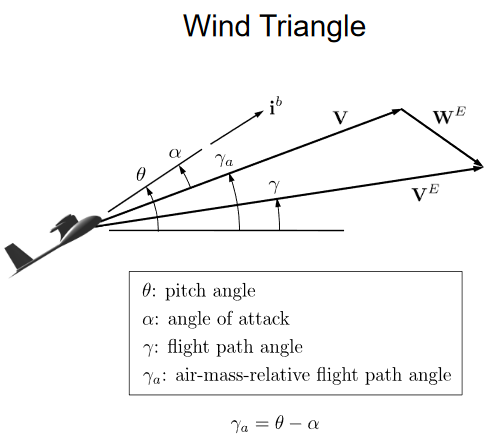
\includegraphics[width=0.75\linewidth]{Images/wind_triangle.png}

\section*{Kinematics and Dynamics}
\begin{tabular}{|l|l|}
\hline
    Name        & Description\\ \hline
    $x_E$       & Intertial x (North) position \\
    $y_E$       & Interial y (East) position \\
    $z_E$       & Inertial z (Down) position \\
    $\phi$      & Roll Angle\\
    $\theta$    & Pitch Angle\\
    $\psi$      & Yaw Angle\\
    $u^E$       & Inertial Velocity along $\hat{i}_B$\\
    $v^E$       & Inertial Velocity along $\hat{j}_B$\\
    $w^E$       & Inertial Velocity along $\hat{k}_B$\\
    $p$         & Angular Velocity along $\hat{i}_B$ (Roll rate)\\
    $q$         & Angular Velocity along $\hat{j}_B$ (Pitch rate)\\
    $r$         & Angular Velocity along $\hat{k}_B$ (Yaw rate)\\ \hline
\end{tabular}
% Pick up at lecture 4

\end{multicols*}  
\end{document}